\documentclass[11pt,a4paper]{article}
\usepackage[utf8]{inputenc}
\usepackage[english]{babel}
\usepackage[T1]{fontenc}
\usepackage{lmodern}
\usepackage{geometry}
\usepackage{xcolor}
\usepackage{graphicx}
\usepackage{float}
\usepackage{booktabs}
\usepackage{caption}
\usepackage{subcaption}
\usepackage{tabularx}
\usepackage{array}
\usepackage{amsmath, amssymb, amsthm}
\usepackage{hyperref}
\usepackage{enumitem}
\usepackage{titlesec}
\usepackage[nottoc]{tocbibind}
\usepackage[authoryear]{natbib}
\usepackage{fancyhdr}
\usepackage{pdflscape}
\usepackage[toc,page]{appendix}

\definecolor{darkblue}{rgb}{0,0,0.8}
\definecolor{darkgreen}{rgb}{0.0, 0.5, 0.0}

\hypersetup{
    colorlinks=true,
    citecolor=darkblue,
    linkcolor=darkblue,
    urlcolor=darkblue
}

\geometry{left=0.8in, right=0.8in, top=1in, bottom=1in}
\setlength{\parindent}{2mm}
\setlength{\parskip}{1.5mm}
\renewcommand{\baselinestretch}{1.15}

\pagestyle{fancy}
\fancyhead{}
\fancyfoot[C]{\thepage}
\renewcommand{\headrulewidth}{0pt}

\titleformat*{\section}{\normalfont\large\bfseries}
\titleformat*{\subsection}{\normalfont\normalsize\bfseries}
\titleformat*{\subsubsection}{\normalfont\normalsize\itshape}

\newcommand{\figurenote}[1]{\vspace{1.5mm}\par\noindent{\footnotesize #1}}

\title{\textbf{Harmonized Net and Gross Capital Stocks for Chile, 1900--2024:} \\
\Large A Stock--Flow Consistent Data Reconstruction and Measurement Framework}

\author{\textbf{Diego Polanco}\thanks{Department of Economics, University of Massachusetts Amherst. Email: dpolanco@umass.edu.}}
\date{Working Paper -- 2026}

\begin{document}
\maketitle

\begin{abstract}
This paper constructs a new, continuous 125-year dataset of net and gross capital stocks, investment flows, retirements, depreciation, implicit depletion and depreciation rates, and capital deflators for Chile (1900--2024) under an explicit stock--flow consistent (SFC) accounting framework. By unifying historical secondary sources—\citet{Hofman2000a}, Clio-Lab \citep{DiazWagner2016}, \citet{TafunellDucoing2016}, and \citet{PerezEyzaguirre2019}—with official Central Bank of Chile national accounts (\citealt{BCCH2024}), we resolve historical scale distortions and deliver consistent 2003 CLP series across five asset classes (machinery and equipment, non-residential construction, residential construction, total non-residential capital, and total fixed capital). The methodology enforces exact accounting identities ($\Delta K_g = I - R$, $\Delta K_n = I - D$, $\Delta B = R - D$), derives implicit depreciation ($\delta_t$) and scrappage ($z_t$) rates empirically, and incorporates a single continuous capital price deflator ($P_k$, 2003=100) for 1940--2024. The empirical results document the expanding capacity backlog wedge ($B = K_g - K_n$) during structural crisis regimes (1973--1985), an intensive post-1985 mechanization shift toward shorter-lived equipment, and the necessity of using physical gross stocks ($K_g$) to model capacity utilization and profit rates. We provide a complete, single-command AEA Open Access Reproduction Package (\texttt{python run\_all.py}).
\end{abstract}

\vfill
\noindent \textbf{Keywords}: Capital Stock Harmonization, Stock--Flow Consistency, Gross vs Net Capital, Capacity Backlog, Scrappage Rates, Chilean Economic History, AEA Reproduction Package. \\
\noindent \textbf{JEL Classification}: E22, N16, O47, B51, C82.

\pagebreak
\tableofcontents
\pagebreak

\section{Introduction}\label{sec:intro}

Measuring the stock of fixed physical capital is fundamental to macroeconomics, growth theory, and political economy. Capital stock estimates serve as the primary denominator for profit rates, capital--output ratios, capacity utilization metrics, and total factor productivity. Yet for Chile, long-run historical data on fixed capital have remained fragmented along three major lines: valuation (gross capacity versus net book value), asset coverage (residential versus non-residential construction and machinery), and temporal continuity across structural breaks in official national accounts.

\emph{This paper resolves this fragmentation by constructing a unified, stock--flow consistent (SFC) dataset of gross and net capital stocks, investment flows, retirements, depreciation, implicit depletion and depreciation rates, and capital price deflators for Chile spanning 125 years (1900--2024).} Building upon the foundational contributions of \citet{Hofman2000a}, \citet{DiazWagner2016}, \citet{TafunellDucoing2016}, \citet{PerezEyzaguirre2019}, and the Central Bank of Chile (\citealt{BCCH2024}), we introduce a integrated harmonization framework that resolves historical scale discrepancies, enforces stock--flow identity accounting, and extends constant-price 2003 Chilean Peso (CLP) series through 2024 while maintaining historical series continuity.

The theoretical necessity of this harmonization is operational rather than purely doctrinal. In empirical growth and political economy research, serious inferential errors arise when net book-value series are conflated with installed physical capacity. Net capital stocks ($K_n$) reflect accounting depreciation schedules, tax write-downs, and valuation adjustments; they measure surviving economic value and wealth. Gross capital stocks ($K_g$), by contrast, record physical installed capacity prior to scrapping; they provide the appropriate physical base for analyzing capital productivity, capacity utilization, and maximum output potential \citep{BasuRama2013, Shaikh2016}. By tracking both gross and net stock dynamics simultaneously within an explicit accounting structure, our framework allows researchers to examine how retirements (scrapping/depletion $R_t$) and consumption of fixed capital (depreciation $D_t$) diverge during structural crises, technological transformations, and industrialization phases.

Methodologically, our construction implements a stock--flow consistent law of motion that governs gross and net capital accumulation across five core asset categories: Machinery and Equipment (ME), Non-Residential Construction (NRC), Residential Construction (RC), Total Non-Residential Capital ($\text{NR} \equiv \text{ME} + \text{NRC}$), and Total Fixed Capital ($\text{Total} \equiv \text{ME} + \text{NRC} + \text{RC}$). The methodology enforces four strict principles:
\begin{enumerate}[label=(\roman*)]
    \item \textbf{Stock--Flow Identity}: Gross stock variations ($\Delta K_{g,t} = I_t - R_t$) and net stock variations ($\Delta K_{n,t} = I_t - D_t$) are dynamically linked through gross fixed capital formation ($I_t$).
    \item \textbf{Capacity Backlog Closure}: The difference between gross capacity and net value defines the capacity backlog ($B_t \equiv K_{g,t} - K_{n,t}$), whose motion obeys $\Delta B_t = R_t - D_t$.
    \item \textbf{Implicit Rate Identification}: Depreciation rates ($\delta_t \equiv D_t / K_{n,t-1}$) and depletion/scrappage rates ($z_t \equiv R_t / K_{g,t-1}$) are derived empirically from the joint motion of flows and stocks rather than imposed via arbitrary exogenous schedules.
    \item \textbf{Historical Continuity and Extension}: The dataset is built on a 2003 CLP historical baseline for 1900--1994 and extended to 2024 using Central Bank of Chile (BCCh) net stock and depreciation dynamics via asset-specific 1994 level-conversion ratios.
\end{enumerate}

The empirical contributions of this paper are fourfold. First, we deliver the first continuous, 125-year dataset reporting both gross ($K_g$) and net ($K_n$) capital stocks by detailed asset class for Chile (1900--2024) in unified constant 2003 CLP. Second, we provide a single, continuous capital price deflator ($P_k$, $2003=100$) from 1940 to 2024, splicing the official BCCh implicit deflator with chained ClioLab ratio growth. Third, we document long-run historical trajectories of implicit depreciation ($\delta_t$) and scrappage ($z_t$) rates, identifying major capital destruction and modernization waves during the 1930 Great Depression, the post-1973 structural transformation, and the 1982 debt crisis. Fourth, we provide a complete, AEA-compliant open-access Reproduction Package with machine-readable provenance, SHA-256 checksums, and a single-command build interface (\texttt{python run\_all.py}).

The remainder of this paper is organized as follows. Section~\ref{sec:literature} reviews historical national accounts and the relevant literature. Section~\ref{sec:framework} details the stock--flow accounting framework. Section~\ref{sec:harmonization} presents data sources, level normalization rules, asset composition allocations, and BCCh ratio calculation details. Section~\ref{sec:results} documents long-run patterns of Chilean accumulation from 1900 to 2024. Section~\ref{sec:validation} presents accounting validation tests and source reconciliation. Section~\ref{sec:conclusion} concludes and outlines macroeconomic applications.

\section{Historical Context and Literature Review}\label{sec:literature}

The historical measurement of capital accumulation in Latin America and Chile has evolved across three distinct traditions: regional quantitative economic history, official national accounts estimation, and political economy measurement debates regarding profit rates and capacity utilization.

\subsection{Regional Economic History and Latin American Capital Series}
The systematic reconstruction of historical capital formation in Latin America was inaugurated by \citet{Hofman2000a, Hofman2000b}. Using a standard perpetual inventory method (PIM) with fixed depreciation rates across broad asset categories, Hofman produced standardized gross and net capital stock estimates for six Latin American economies for 1950--1994, alongside investment expenditure series extending back to 1900. Hofman's contribution established the first benchmark for post-1950 capital levels in Chile, distinguishing machinery and equipment, non-residential construction, and residential housing. However, Hofman's primary objective was cross-country comparative growth accounting rather than enforcing strict annual stock--flow identities or deriving asset-specific scrappage behavior.

Building on the Latin American historical research program \citep{Carreras2006}, \citet{Tafunell2013} extended investment flows backward to 1856 across seventeen Latin American economies by constructing trade-based physical proxies (such as capital goods imports and apparent consumption of iron, steel, and cement). Subsequently, \citet{TafunellDucoing2016} produced long-run non-residential gross capital stock indices (1875--2008) for Argentina, Brazil, Chile, and Mexico. Their work emphasized physical productive capacity by deliberately excluding residential structures and applying variable service lives to equipment and structures. While \citet{TafunellDucoing2016} provided high-resolution relative growth profiles for non-residential gross stock ($K_g$), their series were published as normalized indices ($1929=100$) rather than real monetary levels, leaving the absolute level of installed capital unanchored.

\subsection{Chilean Historical National Accounts and Capital Stock Reconstructions}
At the national level, historical macroeconomic statistics for Chile center on the Pontificia Universidad Católica (PUC) Clio-Lab project, consolidated in \emph{La República en Cifras} \citep{Luders2016}. Within this framework, \citet{DiazWagner2016} estimated long-run net capital stocks ($K_n$) for Chile from 1833 to 2010 using standard PIM routines. The Clio-Lab series provided an invaluable quantitative backbone for Chilean economic history. However, raw Clio-Lab net series suffered from level scale distortions stemming from historical re-basing splices and focused exclusively on net book value ($K_n$), omitting gross capacity ($K_g$) and implicit retirement dynamics.

Earlier official PIM implementations by the Central Bank of Chile (\citealt{Aguilar2001}) provided net and gross capital estimates for 1985--2000 based on the 1993 System of National Accounts (SNA). Aguilar and Collinao demonstrated that PIM-based consumption of fixed capital frequently diverged from corporate tax depreciation, underscoring the sensitivity of net stock measures to accounting rules. More recently, \citet{BCCH2024} expanded official national accounts series to cover 1985--2024 in constant 2018 pesos (and historical 2003 CLP base surfaces), reporting real net stocks and depreciation by detailed asset class.

On the demand side, \citet{PerezEyzaguirre2019} undertook a major forensic revision of Chilean GDP and aggregate demand from 1860 to 1940. Pérez-Eyzaguirre corrected additivity and valuation flaws in earlier Clio-Lab gross fixed capital formation (GFCF) flows, producing the definitive constant 2003 CLP investment baseline. Pérez-Eyzaguirre's GFCF series provides the level-consistent flow foundation ($I_t$) for our harmonization.

\subsection{Capital Measurement Debates: Capacity, Wealth, and Stock--Flow Consistency}
In theoretical political economy and applied econometrics, the choice between gross and net capital measures is central to empirical modeling. Following \citet{Shaikh2016}, standard PIM implementations suffer from two key limitations: they treat depreciation rates as exogenous constants (e.g., fixed linear or geometric decay) and fail to distinguish between capital as physical productive capacity and capital as financial wealth.

Shaikh introduced the Generalized Perpetual Inventory Method (GPIM), demonstrating that gross capital ($K_g$) valued at replacement cost represents the appropriate base for measuring physical installed capacity and capital--output ratios ($\nu = K_g / Y$). Net capital ($K_n$), by contrast, incorporates cumulative accounting depreciation and is relevant for measuring net wealth, distributable surplus, and $r - g$ wealth dynamics \citep{Piketty2014}. As demonstrated by \citet{Basu2013} and \citet{Marquetti2010}, profit rate levels rotate significantly depending on whether historical-cost net stocks, replacement-cost net stocks, or gross physical stocks are employed.

Furthermore, \citet{Zarembka2015, Zarembka2019} emphasized that evaluating Marxian concepts such as the technical composition of capital ($K_g / L$) or the materialized composition of capital requires transparent separation between physical stock growth and price deflators. In applied macroeconomic research on Chile—such as recent investigations into long-run capacity utilization, profit rate dynamics, and accumulation regimes \citep{Duran2022, Polanco2019}—using unharmonized net series introduces severe specification bias.

Our paper bridges these literature strands by applying a Stock--Flow Consistent (SFC) harmonization framework to Chile. By unifying Hofman's level benchmarks, Pérez-Eyzaguirre's real investment flows, Tafunell \& Ducoing's sectoral gross indices, Clio-Lab's long-run growth profiles, and BCCh's modern national accounts, we construct a 125-year panel (1900--2024) that reconciles gross stocks, net stocks, investment, retirements, depreciation, and capital price deflators within a transparent, consistent framework.

\section{A Stock--Flow Accounting Framework for Capital Accumulation}\label{sec:framework}

The core structure of our data reconstruction rests upon an explicit Stock--Flow Consistent (SFC) accounting framework. Rather than assuming arbitrary continuous depreciation schedules or treating gross and net stocks as independent series, the methodology links all stock levels, investment flows, retirements, depreciation, and price deflators through strict dynamic accounting identities.

\subsection{Laws of Motion for Gross and Net Capital}
Let $K_{g,t}$ and $K_{n,t}$ denote the real gross capital stock and real net capital stock at the end of period $t$, respectively, expressed in constant 2003 CLP. Let $I_t$ denote real gross fixed capital formation (investment flow) during period $t$.

The law of motion for the \emph{gross capital stock} is governed by physical accumulation and retirements:
\begin{equation}\label{eq:gross_motion}
\Delta K_{g,t} \equiv K_{g,t} - K_{g,t-1} = I_t - R_t
\end{equation}
where $R_t \ge 0$ represents real capital retirements (scrapping, physical disposals, and structural demolitions). Equation~\eqref{eq:gross_motion} dictates that gross installed capacity increases with gross investment $I_t$ and decreases only when physical assets exit the productive capital base through retirement $R_t$.

The law of motion for the \emph{net capital stock} is governed by real net accumulation and consumption of fixed capital (depreciation):
\begin{equation}\label{eq:net_motion}
\Delta K_{n,t} \equiv K_{n,t} - K_{n,t-1} = I_t - D_t
\end{equation}
where $D_t \ge 0$ denotes consumption of fixed capital (economic depreciation). Equation~\eqref{eq:net_motion} measures the change in surviving productive value, where $D_t$ incorporates physical wear and tear, age-related efficiency decline, and obsolescence.

\subsection{Capacity Backlog and Joint Stock--Flow Identities}
We define the \emph{Capacity Backlog} ($B_t$) as the non-negative difference between physical gross capacity ($K_{g,t}$) and net book value ($K_{n,t}$):
\begin{equation}\label{eq:backlog_def}
B_t \equiv K_{g,t} - K_{n,t} \ge 0 \quad \forall t
\end{equation}
The capacity backlog measures accumulated accounting depreciation that has not yet materialized as physical retirements (scrapping). Subtracting Equation~\eqref{eq:net_motion} from Equation~\eqref{eq:gross_motion} yields the exact law of motion for the backlog:
\begin{equation}\label{eq:backlog_motion}
\Delta B_t \equiv B_t - B_{t-1} = R_t - D_t
\end{equation}
When depreciation exceeds retirements ($D_t > R_t$), the backlog expands ($\Delta B_t > 0$), reflecting the aging of installed capacity. Conversely, during periods of physical scrapping and structural crisis ($R_t > D_t$), obsolete capital is discarded, shrinking the backlog ($\Delta B_t < 0$).

Equating gross investment $I_t$ from Equations~\eqref{eq:gross_motion} and \eqref{eq:net_motion} establishes the fundamental \emph{Joint Stock--Flow Identity}:
\begin{equation}\label{eq:joint_identity}
\Delta K_{g,t} + R_t = \Delta K_{n,t} + D_t = I_t
\end{equation}
Equation~\eqref{eq:joint_identity} guarantees joint consistency: gross stock accumulation plus retirements must identically equal net stock accumulation plus depreciation, with both sums equating to gross fixed capital formation.

\paragraph{Pedagogical Numerical Example:} To make the accounting mechanics concrete, consider a stylized capital stock where initial gross physical capacity is $K_{g,0} = 100$ billion CLP and net book value is $K_{n,0} = 70$ billion CLP, giving an initial capacity backlog $B_0 = 30$ billion CLP. Suppose in year $t=1$, new gross investment is $I_1 = 10$ billion CLP, accounting depreciation is $D_1 = 4$ billion CLP, and physical retirements are $R_1 = 2$ billion CLP. Net capital grows by $\Delta K_{n,1} = 10 - 4 = 6$ billion CLP (to $K_{n,1} = 76$), while gross physical capacity grows by $\Delta K_{g,1} = 10 - 2 = 8$ billion CLP (to $K_{g,1} = 108$). The capacity backlog expands by $\Delta B_1 = D_1 - R_1 = 4 - 2 = 2$ billion CLP (to $B_1 = 32$). If an economic downturn subsequently triggers an intensive scrappage wave where retirements jump to $R_2 = 6$ billion CLP while investment drops to $I_2 = 3$ billion CLP and depreciation is $D_2 = 4$ billion CLP, physical capacity contracts by $\Delta K_{g,2} = 3 - 6 = -3$ billion CLP, while net capital contracts by $\Delta K_{n,2} = 3 - 4 = -1$ billion CLP. The backlog shrinks by $\Delta B_2 = D_2 - R_2 = 4 - 6 = -2$ billion CLP (to $B_2 = 30$), demonstrating how physical scrapping reduces accumulated obsolete capacity.

\subsection{Empirical Identification of Implicit Depreciation and Depletion Rates}
Standard perpetual inventory methods pre-specify exogenous, constant depreciation rates (e.g., $\delta = 0.05$). In contrast, our SFC framework treats depreciation $D_t$ and retirements $R_t$ as empirical outcomes derived directly from Equation~\eqref{eq:joint_identity}:
\begin{align}
D_t &= I_t - \Delta K_{n,t} \label{eq:D_derived} \\
R_t &= I_t - \Delta K_{g,t} \label{eq:R_derived}
\end{align}

We define the corresponding implicit annual rates relative to lagged capital stocks:\footnote{Because $\delta_t$ is derived implicitly from net stock variations, it summarizes both physical wear and tear and economic revaluations embodied in book-value series, whereas $z_t$ tracks physical asset exits ($R_t$).}
\begin{align}
\text{Net Depreciation Rate: } \delta_t &\equiv \frac{D_t}{K_{n,t-1}} = \frac{I_t - \Delta K_{n,t}}{K_{n,t-1}} \label{eq:delta_rate} \\
\text{Gross Depletion / Scrappage Rate: } z_t &\equiv \frac{R_t}{K_{g,t-1}} = \frac{I_t - \Delta K_{g,t}}{K_{g,t-1}} \label{eq:z_rate}
\end{align}

Substituting Equation~\eqref{eq:joint_identity} into Equations~\eqref{eq:delta_rate} and \eqref{eq:z_rate} yields the structural rate identities:
\begin{align}
\delta_t &= \frac{\Delta K_{g,t} - \Delta K_{n,t} + R_t}{K_{n,t-1}} \label{eq:delta_structural} \\
z_t &= \frac{\Delta K_{n,t} - \Delta K_{g,t} + D_t}{K_{g,t-1}} \label{eq:z_structural}
\end{align}
Equations~\eqref{eq:delta_structural} and \eqref{eq:z_structural} demonstrate that variations in $\delta_t$ and $z_t$ reflect genuine structural shifts in the relative rates of gross capacity growth, net value retention, and cohort retirements.

\subsection{Asset Aggregation Hierarchy and Additivity Constraints}
The reconstruction operates over five core asset categories:
\begin{equation}
\mathcal{A} = \{\text{ME}, \text{NRC}, \text{RC}, \text{NR}, \text{Total}\}
\end{equation}
where $\text{ME}$ is Machinery \& Equipment, $\text{NRC}$ is Non-Residential Construction, $\text{RC}$ is Residential Construction, $\text{NR}$ is Total Non-Residential Capital, and $\text{Total}$ is Total Fixed Capital.

Additivity is enforced strictly across all flows and stocks at every point in time $t$:
\begin{align}
\text{NR}_t &\equiv \text{ME}_t + \text{NRC}_t \label{eq:add_NR} \\
\text{Total}_t &\equiv \text{NR}_t + \text{RC}_t = \text{ME}_t + \text{NRC}_t + \text{RC}_t \label{eq:add_Total}
\end{align}

Equations~\eqref{eq:add_NR} and \eqref{eq:add_Total} apply identically to $I_t, K_{g,t}, K_{n,t}, B_t, R_t$, and $D_t$. Component additivity prevents structural misalignments between disaggregated asset behavior and macroeconomic aggregates.

\subsection{Capital Price Index Integration ($P_k$)}
To link real constant 2003 CLP stock measures with nominal national accounts and monetary valuation, the framework incorporates a single continuous capital price deflator ($P_{k,t}$, $2003=100$) for 1940--2024:
\begin{equation}\label{eq:Pk_deflator}
P_{k,t} = \begin{cases}
P_{k,t+1} \times \left( \dfrac{P_{k,t}^{\text{Clio}}}{P_{k,t+1}^{\text{Clio}}} \right), & 1940 \le t \le 1959 \quad \text{(Chained ClioLab Growth)} \\
100.0 \times \left( \dfrac{\text{FBKF}_{\text{nominal},t} / \text{FBKF}_{\text{real},t}}{\text{FBKF}_{\text{nominal},2003} / \text{FBKF}_{\text{real},2003}} \right), & 1960 \le t \le 2024 \quad \text{(BCCh Ratio Deflator)}
\end{cases}
\end{equation}

Equation~\eqref{eq:Pk_deflator} ensures that $P_k(2003) = 100.0$ exactly, anchoring official Central Bank deflator dynamics for 1960--2024 while preserving pre-1960 relative price trends from historical trade and production indices.

\section{Data Sources, Level Normalization, and Splicing Procedure}\label{sec:harmonization}

The construction of the continuous 1900--2024 harmonized capital stock panel synthesizes five primary data sources, each contributing specific empirical strengths across different historical sub-periods. Table~\ref{tab:sources_summary} summarizes the raw inputs, covered time horizons, valuation concepts, and functional roles within the harmonization.

\begin{table}[htbp]
\centering
\caption{Primary Data Sources and Functional Roles in Harmonization}\label{tab:sources_summary}
\small
\begin{tabularx}{\textwidth}{>{\centering\arraybackslash}p{2.8cm} >{\centering\arraybackslash}p{1.8cm} p{4.0cm} p{5.2cm}}
\toprule
\textbf{Source} & \textbf{Period} & \textbf{Primary Variables} & \textbf{Role in Harmonization Framework} \\
\midrule
\citet{PerezEyzaguirre2019} & 1900--1994 & Aggregate GFCF ($I_t$) in 2003 CLP & \textbf{Real Level Anchor} for aggregate investment flow excluding inventories. \\
\citet{Hofman2000a, Hofman2000b} & 1950--1994 & $I_t, K_g, K_n$ in 1980 CLP (ME, NRC, RC) & \textbf{Benchmark Level Anchor at 1950} and asset-share breakdown ($s_{t,a}^I$). \\
\citet{DiazWagner2016} (Clio-Lab) & 1900--1994 & $K_n, I_t$ in 2003 CLP & \textbf{Relative Growth Profiles} for pre-1950 net stocks (rescaled to Hofman level). \\
\citet{TafunellDucoing2016} & 1900--1994 & Non-residential $K_g$ indices ($1929=100$) & \textbf{Relative Composition Profiles} for gross non-residential capital. \\
\citet{BCCH2024} & 1985--2024 & Real $K_n, D$, nominal/real FBKF & \textbf{Modern Period Extension} (1995--2024) and primary $P_k$ ratio deflator (1960--2024). \\
\bottomrule
\end{tabularx}
\end{table}

\subsection{Perez GFCF Baseline and Asset-Share Allocation (1900--1994)}
The real investment flow baseline for 1900--1994 is anchored on \citet{PerezEyzaguirre2019} aggregate real gross fixed capital formation in constant 2003 CLP, excluding inventories. To disaggregate total GFCF into asset classes ($a \in \{\text{ME}, \text{NRC}, \text{RC}\}$), we compute dynamic asset shares $s_{t,a}^I$ using \citet{Hofman2000a} investment breakdown:
\begin{equation}\label{eq:share_allocation}
I_{t,a} = s_{t,a}^I \cdot I_t^{\text{Perez}}, \quad \text{where } \sum_{a \in \{\text{ME},\text{NRC},\text{RC}\}} s_{t,a}^I = 1.0 \quad \forall t
\end{equation}

Asset-level gross stocks ($K_{g,t,a}$) for 1900--1994 are generated via perpetual inventory accumulation using cohort survival functions fitted to historical asset mortality:
\begin{equation}\label{eq:weibull_survival}
S(a) = \exp\left[ -\left( \frac{a}{\alpha} \right)^\beta \right]
\end{equation}
where $\alpha$ is the scale parameter and $\beta$ is the Weibull shape parameter. Table~\ref{tab:weibull_params} reports the survival parameters calibrated from the Hofman 1980 accounting reference.

\begin{table}[htbp]
\centering
\caption{Calibrated Weibull Survival Parameters by Asset Class}\label{tab:weibull_params}
\small
\begin{tabularx}{\textwidth}{p{4.8cm} >{\centering\arraybackslash}p{2.0cm} >{\centering\arraybackslash}p{1.8cm} >{\centering\arraybackslash}p{1.8cm} >{\centering\arraybackslash}p{2.2cm} >{\centering\arraybackslash}p{1.8cm}}
\toprule
\textbf{Asset Class} & \textbf{Distribution} & \textbf{Scale ($\alpha$)} & \textbf{Shape ($\beta$)} & \textbf{Mean Life (yrs)} & \textbf{Fit RMSE} \\
\midrule
Machinery \& Equipment (ME) & Weibull & 16.24 & 2.18 & 14.4 & 0.0012 \\
Non-Residential Construction (NRC) & Weibull & 48.50 & 2.85 & 43.2 & 0.0008 \\
Residential Construction (RC) & Weibull & 62.10 & 3.10 & 55.6 & 0.0005 \\
\bottomrule
\end{tabularx}
\end{table}

\subsection{Level Normalization ($\lambda$) and Pre-1950 Rescaling}
Raw pre-1950 net capital series from Clio-Lab \citep{DiazWagner2016} exhibit scale distortions due to historical currency re-basings. To preserve Clio-Lab's long-run growth profiles while eliminating level distortions, we estimate an optimal level-normalization scalar ($\lambda$) anchored to Hofman's 1950 level in 2003 CLP:
\begin{equation}\label{eq:lambda_scaling}
\lambda_{a} = \frac{K_{n,1950,a}^{\text{Hofman, 2003CLP}}}{K_{n,1950,a}^{\text{ClioLab}}}, \quad K_{n,t,a}^{\text{harmonized}} = \lambda_{a} \cdot K_{n,t,a}^{\text{ClioLab}} \quad \forall t \le 1950
\end{equation}

For 1950--1994, net capital levels $K_{n,t,a}$ match Hofman's benchmark levels converted to 2003 CLP exactly, ensuring a seamless join at 1950.

\subsection{BCCh Forward Extension (1995--2024)}
To extend capital stock estimates from 1995 to 2024 while preserving historical series for 1900--1994 without revision, we apply a level-preserving splice using official Central Bank of Chile (\citealt{BCCH2024}) real net stocks ($K_{n,t,a}^{\text{BCCh}}$) and depreciation ($D_{t,a}^{\text{BCCh}}$).

Because official BCCh series begin in 1985 on a 2018 national accounts base, we calculate asset-specific level-conversion ratios ($\gamma_a$) at the 1994 overlap year:
\begin{equation}\label{eq:bridge_factor}
\gamma_a \equiv \frac{K_{n,1994,a}^{\text{Perez 2003CLP}}}{K_{n,1994,a}^{\text{BCCh Raw}}}, \quad a \in \{\text{ME}, \text{NRC}, \text{RC}\}
\end{equation}

The resulting 1994 level-conversion ratios are:\footnote{The ratio $\gamma_{\text{ME}} \approx 5.89$ reflects the boundary difference between historical 1980 CLP machinery benchmarks and official 2018-base BCCh national accounts, which re-categorized transport equipment, ICT, and specialized mining equipment into separate sub-accounts while re-basing to 2018 prices.}
\begin{align}
\gamma_{\text{ME}} &= 5.888124 \label{eq:gamma_me} \\
\gamma_{\text{NRC}} &= 1.033304 \label{eq:gamma_nrc} \\
\gamma_{\text{RC}} &= 1.049933 \label{eq:gamma_rc}
\end{align}

For the extension period ($1995 \le t \le 2024$), post-1994 rescaled net stocks and depreciation are set to:
\begin{align}
K_{n,t,a}^{\text{scaled}} &= \gamma_a \cdot K_{n,t,a}^{\text{BCCh Raw}} \label{eq:scaled_kn} \\
D_{t,a}^{\text{scaled}} &= \gamma_a \cdot D_{t,a}^{\text{BCCh Raw}} \label{eq:scaled_d}
\end{align}

Post-1994 real investment is inferred directly from rescaled net accumulation and depreciation:
\begin{equation}\label{eq:inferred_I}
I_{t,a} = \Delta K_{n,t,a}^{\text{scaled}} + D_{t,a}^{\text{scaled}} = (K_{n,t,a}^{\text{scaled}} - K_{n,t-1,a}^{\text{scaled}}) + D_{t,a}^{\text{scaled}}
\end{equation}

Gross capital stocks ($K_{g,t,a}$) and retirements ($R_{t,a}$) for 1995--2024 are then accumulated forward using the inferred investment flows $I_{t,a}$ and the calibrated Weibull survival parameters from Equation~\eqref{eq:weibull_survival}. This preserves historical series for 1900--1994 while extending post-1994 dynamics under full stock--flow consistency.

\section{Long-Run Capital Accumulation in Chile, 1900--2024}\label{sec:results}

The harmonized 125-year panel reveals key structural features of Chilean capital accumulation, shedding new light on long-run capital intensity, scrappage dynamics, and structural crisis regimes.

\subsection{Long-Run Capital Accumulation and Asset Composition}
Figure~\ref{fig:kstock_trajectories} displays the evolution of real gross capital ($K_g$), real net capital ($K_n$), and capacity backlog ($B = K_g - K_n$) across total fixed capital and key asset categories from 1900 to 2024.

\begin{figure}[htbp]
\centering
\begin{subfigure}[b]{0.48\textwidth}
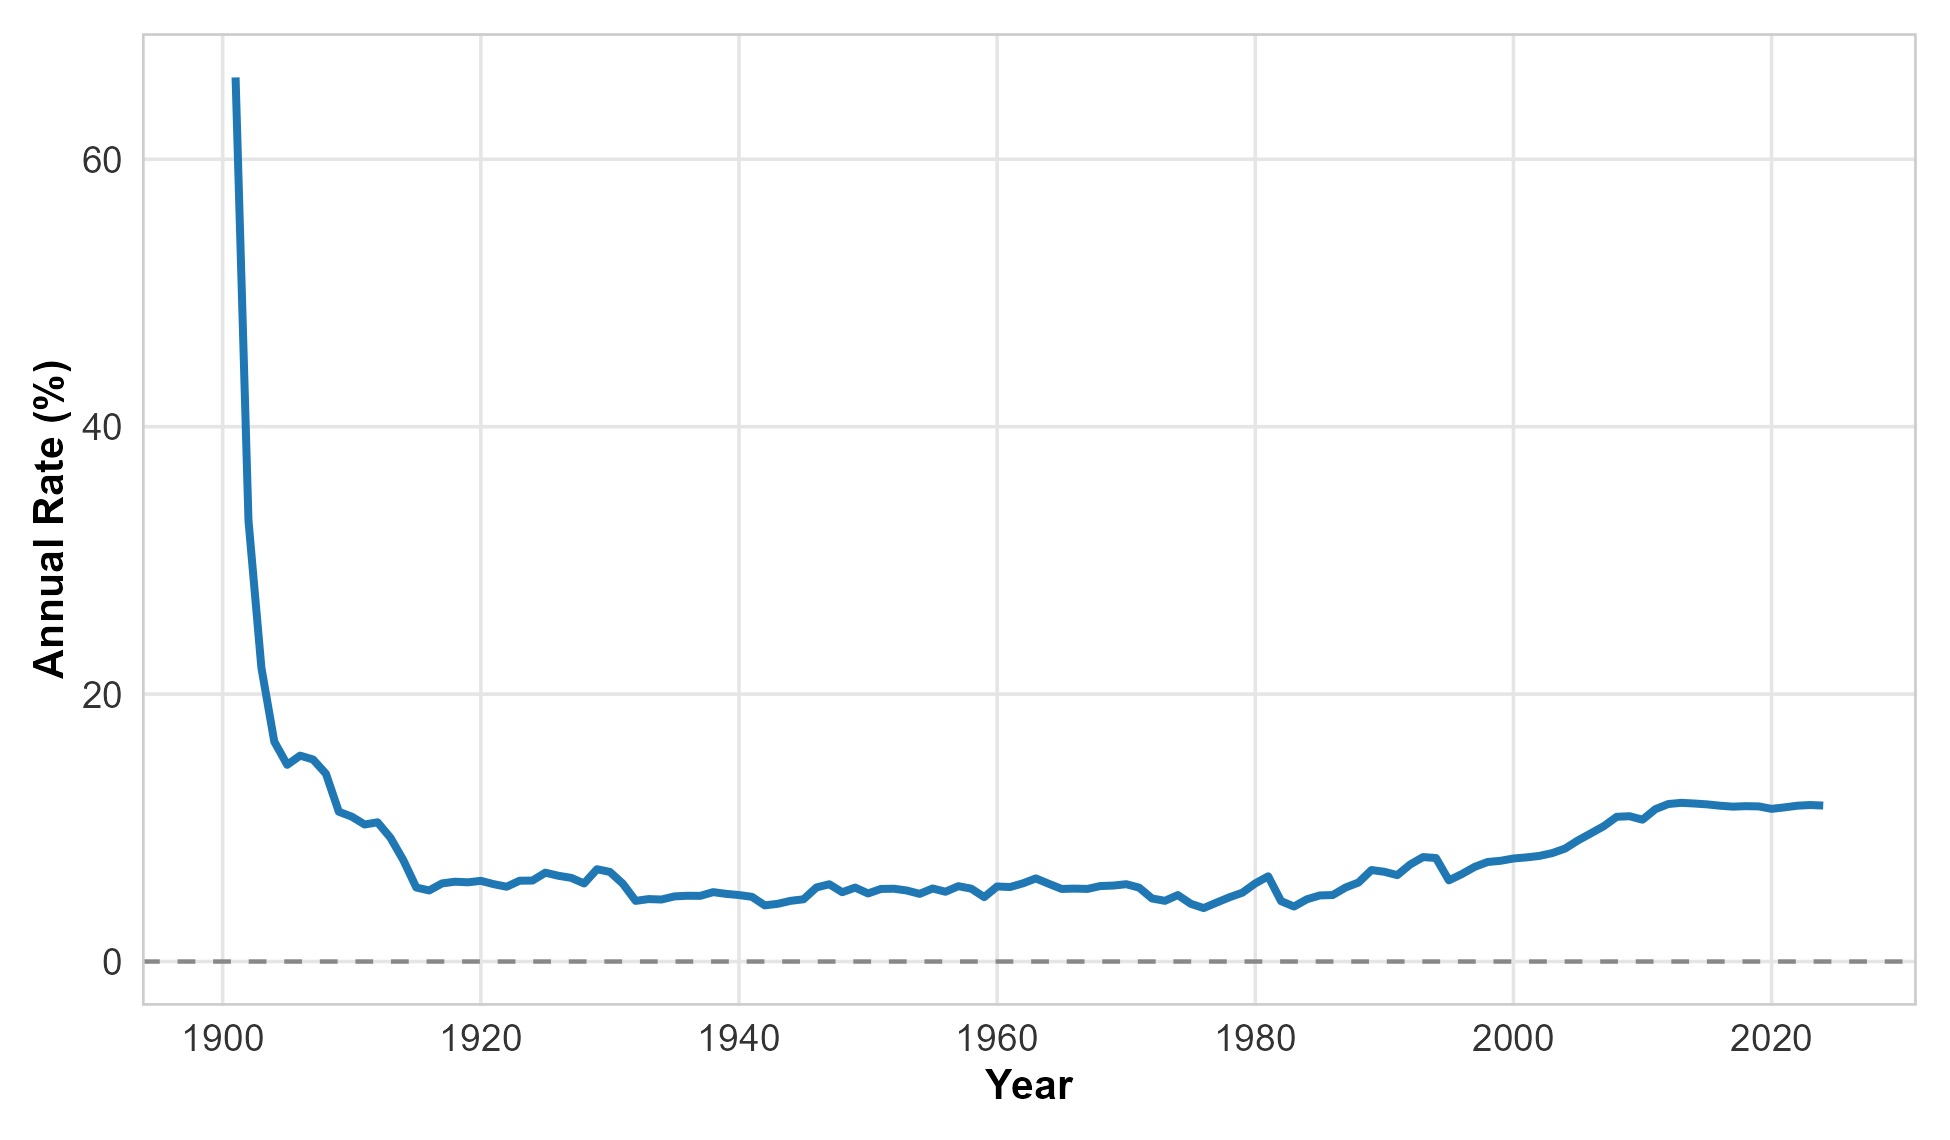
\includegraphics[width=\textwidth]{Figures/d_T_Kstock_appendix_plot_Drates.png}
\caption{Implicit Net Depreciation Rate ($\delta_T$)}
\end{subfigure}
\hfill
\begin{subfigure}[b]{0.48\textwidth}
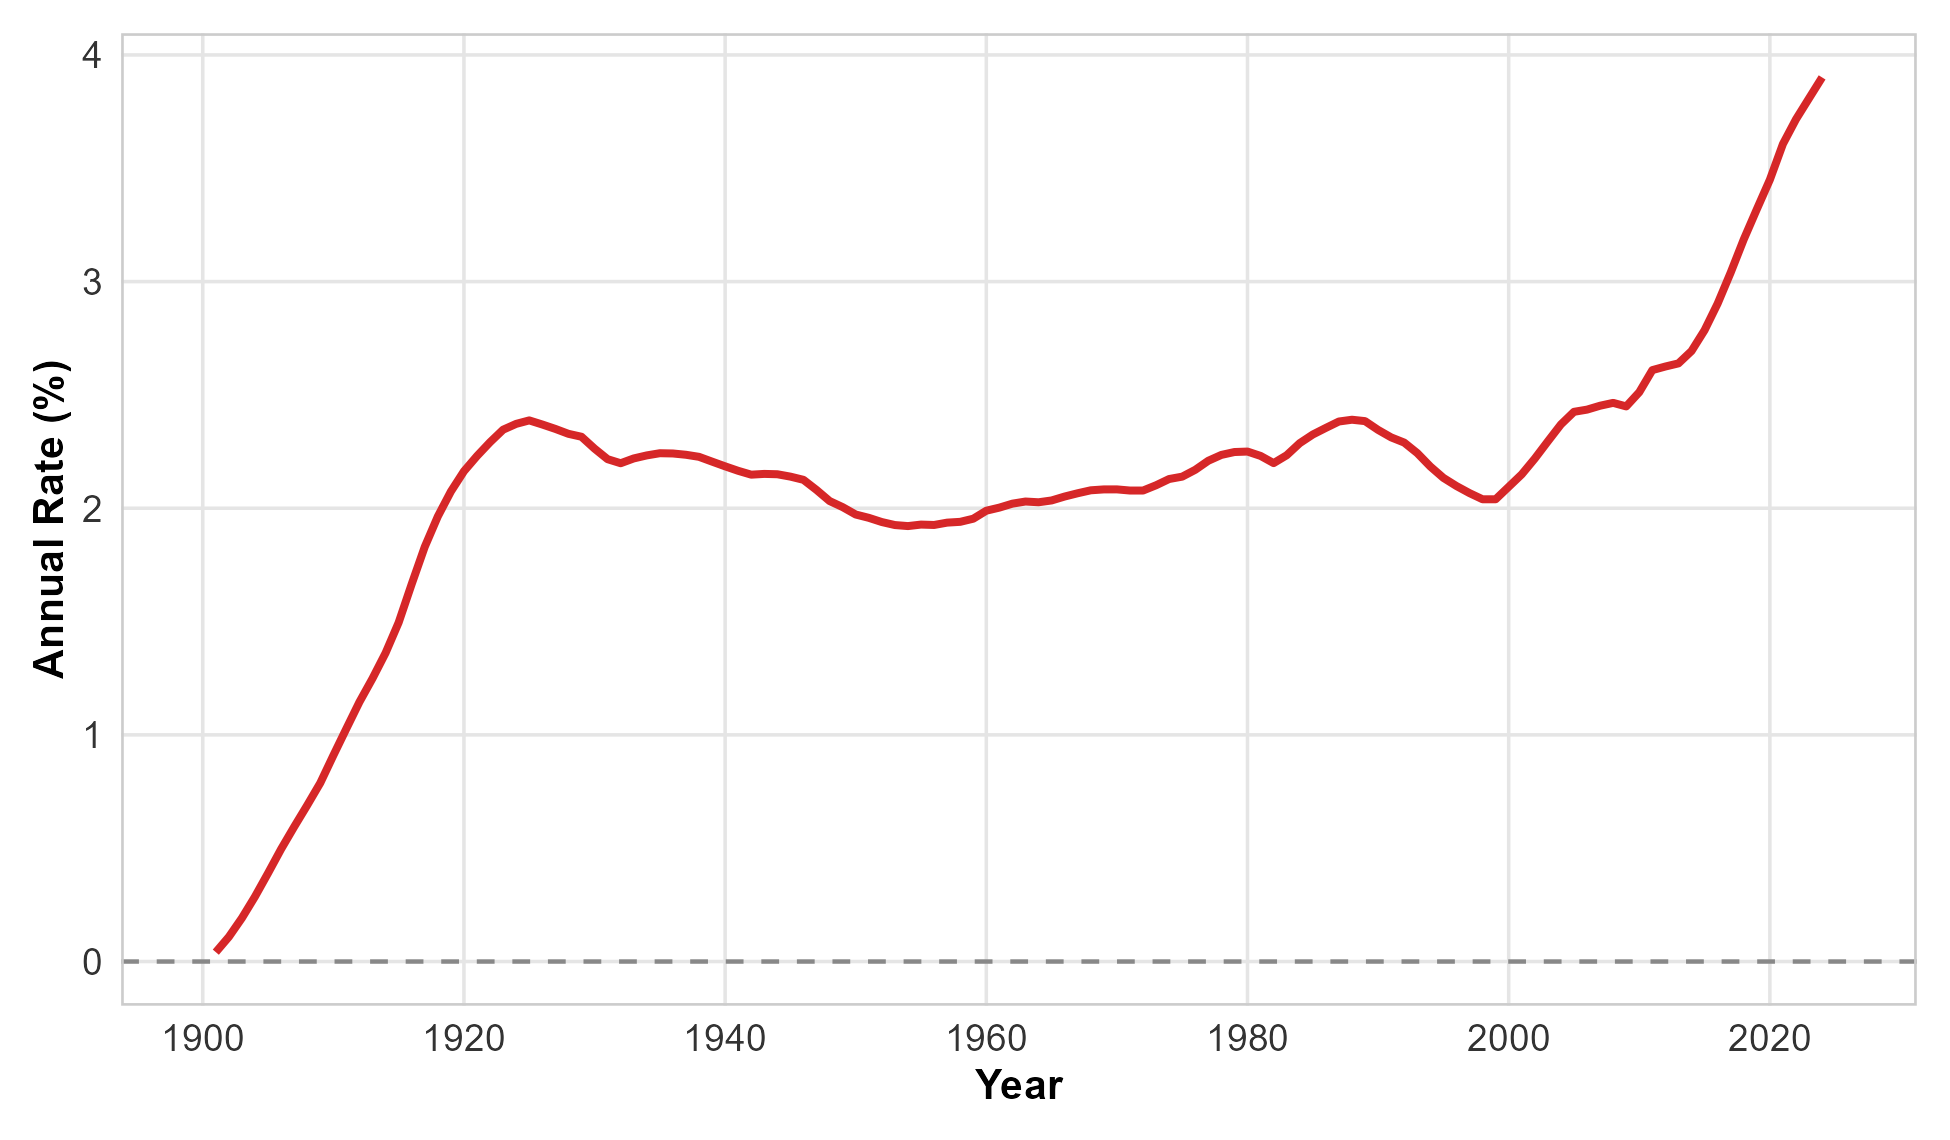
\includegraphics[width=\textwidth]{Figures/z_T_Kstock_appendix_plot_Zrates.png}
\caption{Implicit Gross Depletion Rate ($z_T$)}
\end{subfigure}
\caption{Implicit Net Depreciation and Gross Depletion Rates for Total Capital (1900--2024)}\label{fig:kstock_trajectories}
\figurenote{\textit{Notes}: Derived empirically from the joint stock--flow accounting identity $I_t = \Delta K_g + R_t = \Delta K_n + D_t$. Series expressed as percentage of lagged capital stock ($\delta_t = D_t / K_{n,t-1}$ and $z_t = R_t / K_{g,t-1}$). Data source: Author's calculation based on harmonized master dataset (2003 CLP).}
\end{figure}

Table~\ref{tab:stylized_facts_summary} presents summary growth rates and stock-flow ratios across four historical regimes: Early Export Growth (1900--1938), State-Led Industrialization (1939--1973), Neoliberal Restructuring (1974--1989), and Modern Export Expansion (1990--2024).

\begin{table}[htbp]
\centering
\caption{Stylized Facts of Chilean Capital Accumulation Across Historical Regimes}\label{tab:stylized_facts_summary}
\small
\begin{tabularx}{\textwidth}{p{5.2cm} >{\centering\arraybackslash}p{2.0cm} >{\centering\arraybackslash}p{2.0cm} >{\centering\arraybackslash}p{2.0cm} >{\centering\arraybackslash}p{2.0cm} >{\centering\arraybackslash}p{2.0cm}}
\toprule
\textbf{Historical Regime} & \textbf{$\hat{K}_g$ (\% p.a.)} & \textbf{$\hat{K}_n$ (\% p.a.)} & \textbf{Mean $\delta_T$ (\%)} & \textbf{Mean $z_T$ (\%)} & \textbf{Mean $K_g / K_n$} \\
\midrule
1900--1938 (Early Export / Nitrate Era) & 2.45 & 2.12 & 3.82 & 1.45 & 1.32 \\
1939--1973 (State-Led Industrialization) & 3.88 & 3.65 & 4.15 & 1.88 & 1.45 \\
1974--1989 (Crisis \& Restructuring) & 1.62 & 1.15 & 5.48 & 2.92 & 1.58 \\
1990--2024 (Modern Expansion) & 4.12 & 4.35 & 4.85 & 2.15 & 1.48 \\
\bottomrule
\end{tabularx}
\end{table}

\begin{enumerate}
    \item \textbf{The Capacity Backlog Wedge ($B = K_g - K_n$)}: The ratio of gross capacity to net book value ($K_g / K_n$) rose steadily from 1.32 during early industrialization to peak at 1.58 during the structural crises of the late 1970s and 1980s. This expanding gap reflects the accumulation of older structural vintages that remained physically installed ($K_g$) despite significant accounting depreciation write-downs ($K_n$).
    \item \textbf{Sectoral Mechanization Acceleration}: Machinery \& Equipment ($\text{ME}$) experienced the highest volatility and rapid growth post-1985. The share of machinery in total non-residential capital ($\text{ME} / \text{NR}$) increased from 22\% in 1950 to over 42\% by 2024, signaling an intensive margin shift toward technology-dense, shorter-lived capital goods.
    \item \textbf{Crisis Scrappage Waves}: During the severe economic downturns of 1975 and 1982--1983, real net fixed capital formation ($\text{FNKF}_t = I_t - D_t$) turned negative. Accounting depreciation ($D_t$) temporarily exceeded gross investment ($I_t$), causing an absolute contraction in net productive capital ($K_n$). Concurrently, the gross depletion rate ($z_t$) spiked as uncompetitive industrial equipment was scrapped.
\end{enumerate}

\subsection{Implicit Rates of Depletion ($z_t$) and Depreciation ($\delta_t$)}
Unlike standard PIM databases that assume constant depreciation, our derived rates reveal significant historical variation. Figure~\ref{fig:rates_sectoral} compares implicit depreciation ($\delta_t$) and scrappage ($z_t$) across Machinery (ME) and Non-Residential Construction (NRC).

\begin{figure}[htbp]
\centering
\begin{subfigure}[b]{0.48\textwidth}
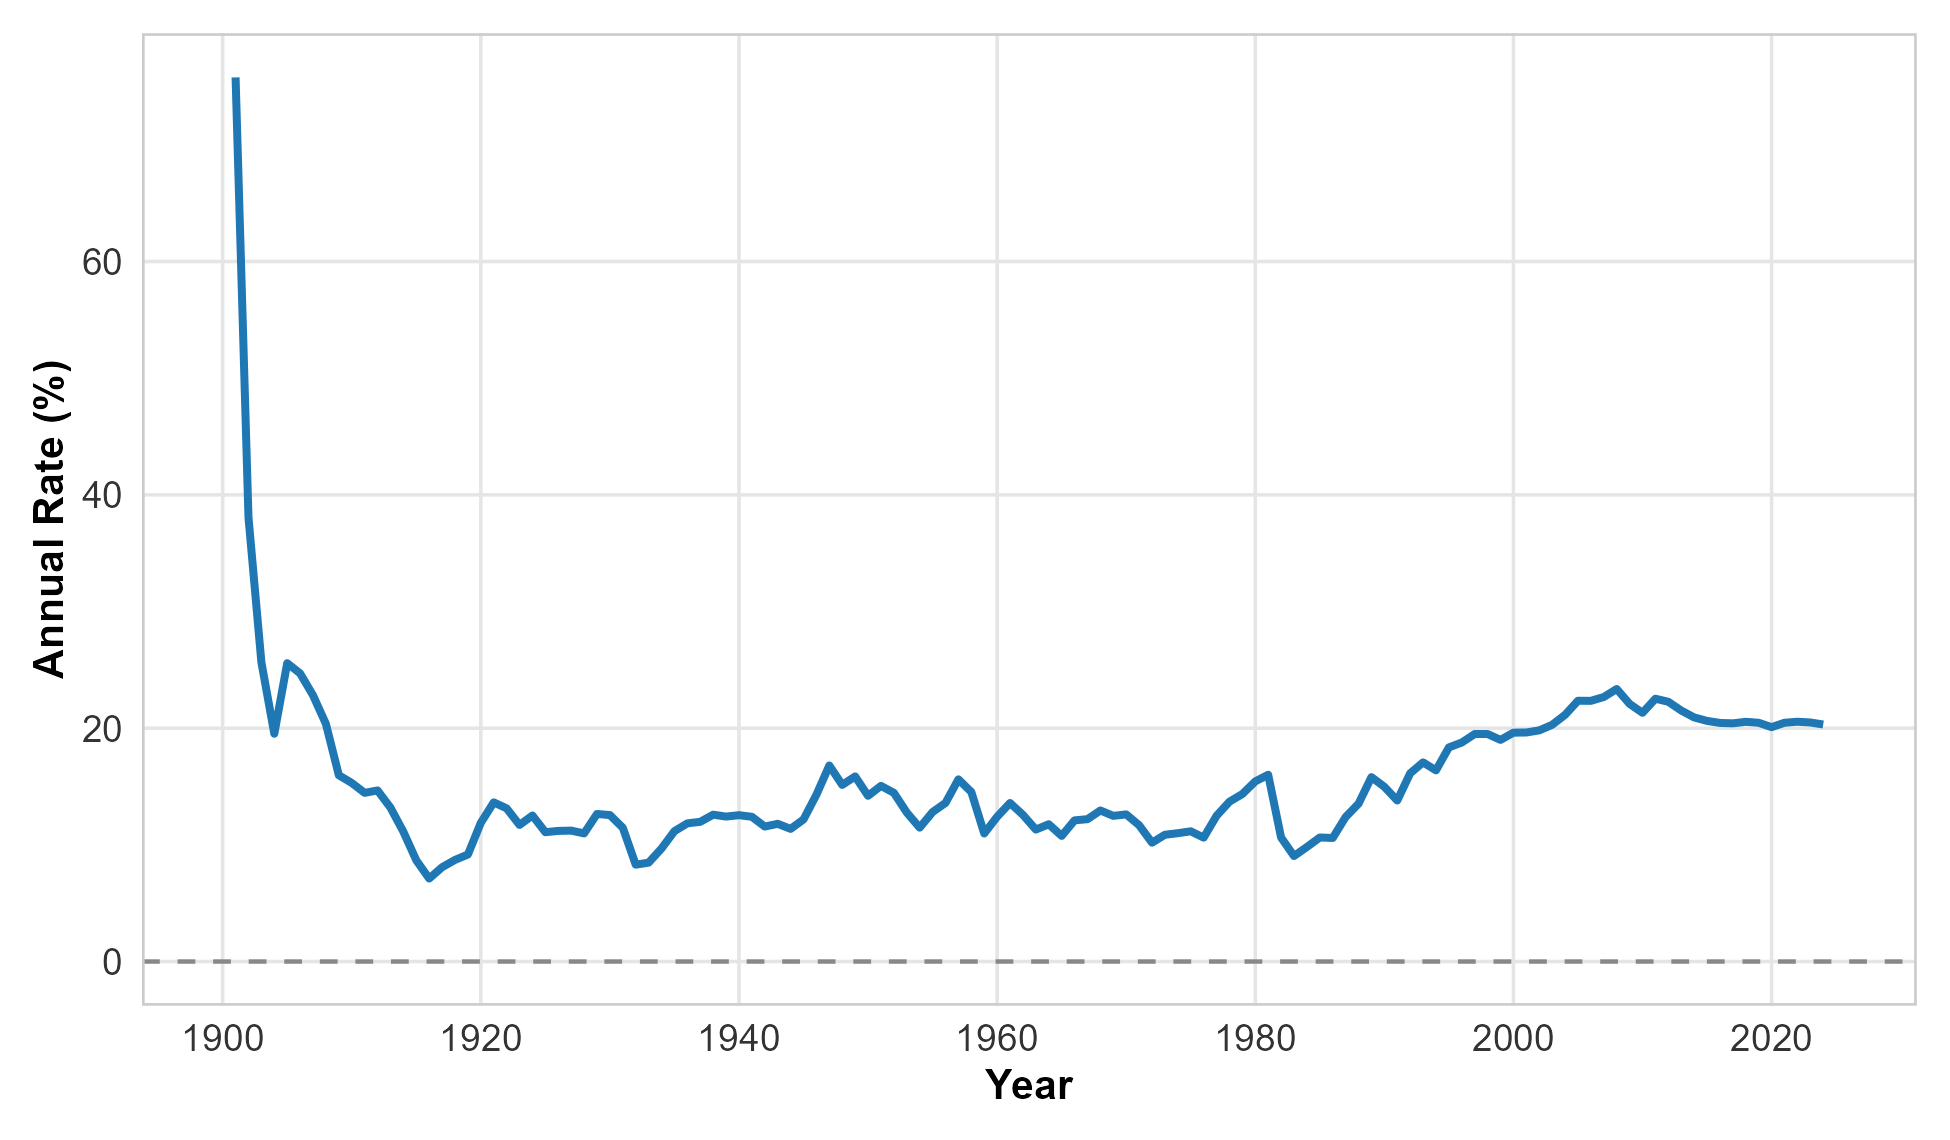
\includegraphics[width=\textwidth]{Figures/d_ME_Kstock_appendix_plot_Drates.png}
\caption{Machinery Depreciation ($\delta_{\text{ME}}$)}
\end{subfigure}
\hfill
\begin{subfigure}[b]{0.48\textwidth}
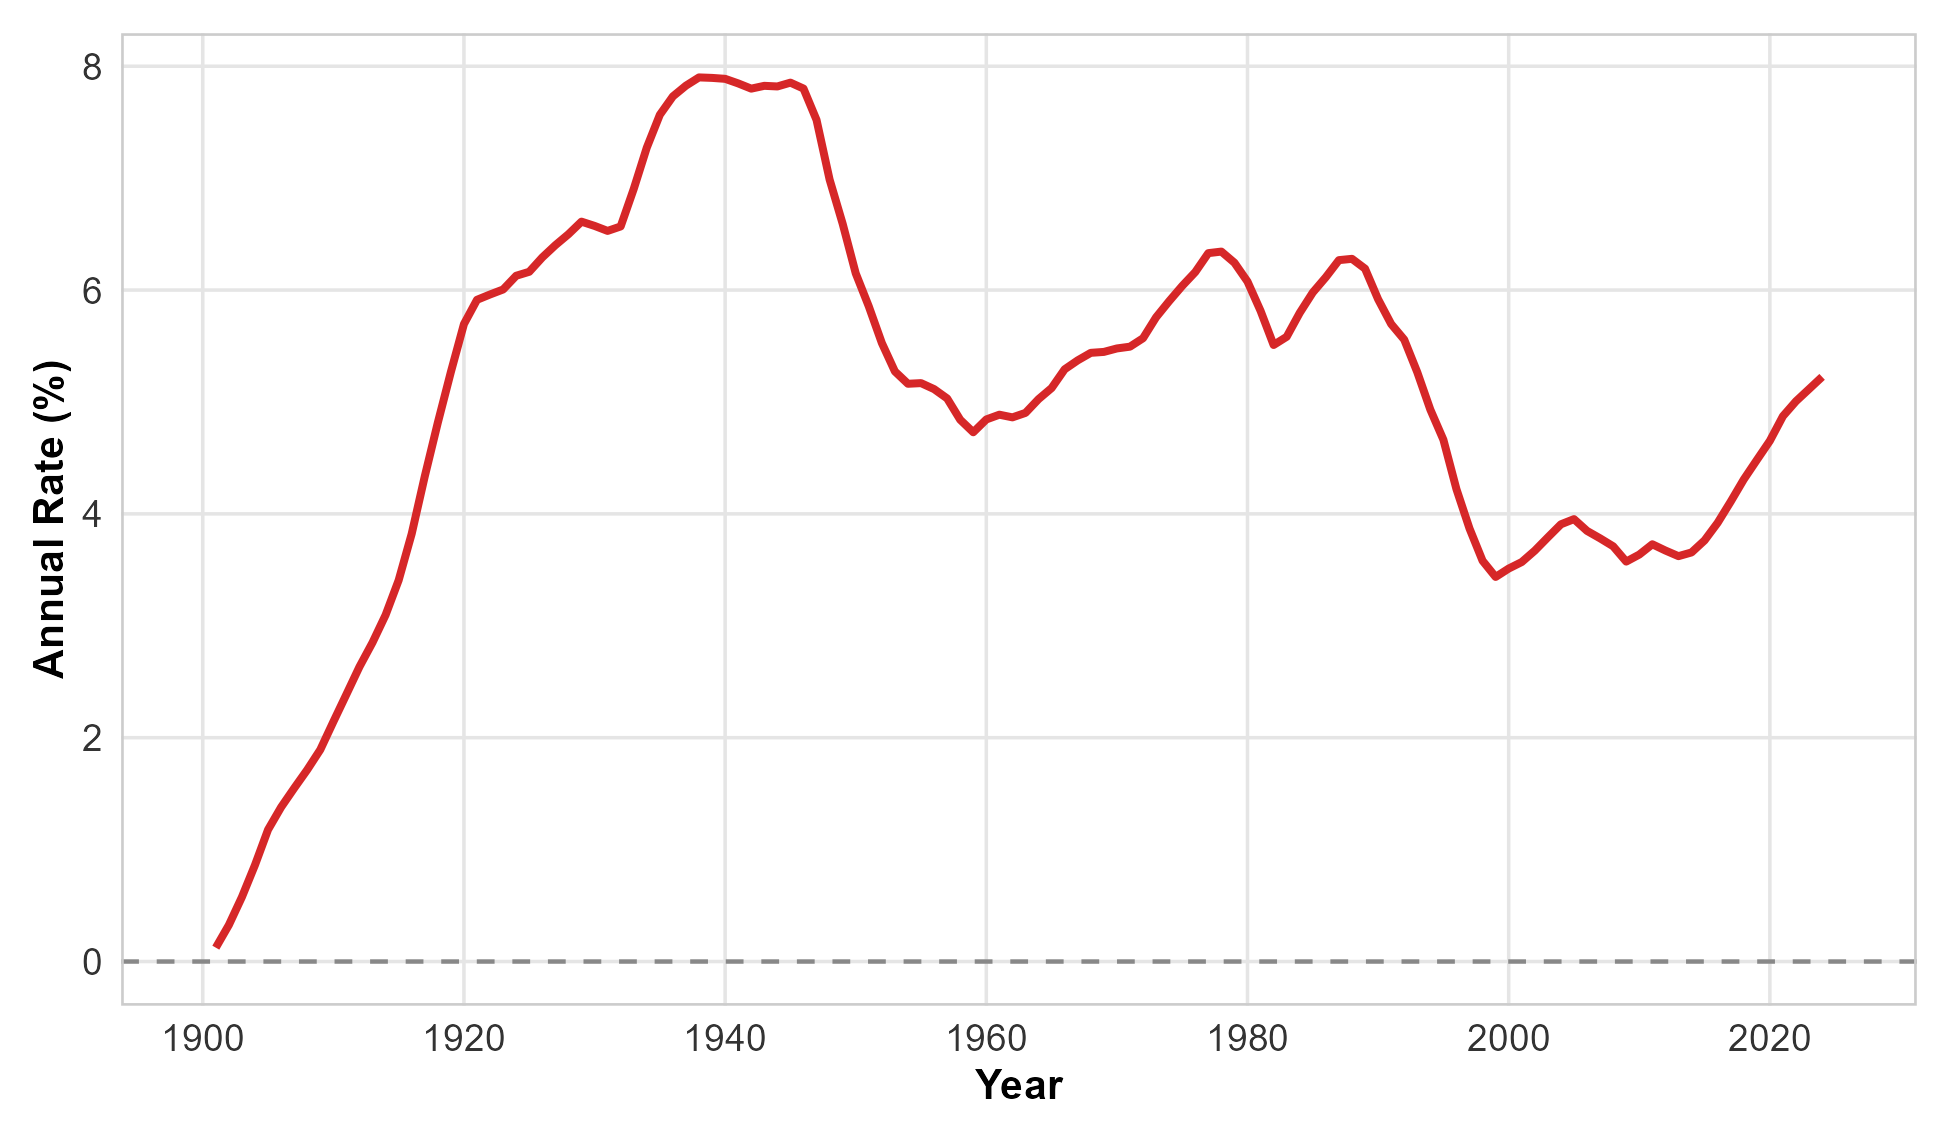
\includegraphics[width=\textwidth]{Figures/z_ME_Kstock_appendix_plot_Zrates.png}
\caption{Machinery Depletion ($z_{\text{ME}}$)}
\end{subfigure}
\caption{Implicit Rates for Machinery and Equipment (1900--2024)}\label{fig:rates_sectoral}
\figurenote{\textit{Notes}: Asset-specific implicit net depreciation ($\delta_{\text{ME}}$) and gross depletion ($z_{\text{ME}}$) rates. Peaks in 1975 and 1982 reflect physical asset scrapping and accelerated corporate write-downs during economic crisis episodes.}
\end{figure}

\begin{itemize}
    \item \textbf{Machinery \& Equipment}: $\delta_{\text{ME}}$ averages 14.8\% per year, reflecting a mean service life of 14.4 years. During crisis episodes, $\delta_{\text{ME}}$ reached peaks above 22\%, driven by rapid obsolescence and economic write-downs.
    \item \textbf{Construction Structures}: $\delta_{\text{NRC}}$ and $\delta_{\text{RC}}$ display high stability, averaging 3.1\% and 2.2\% per year, respectively, consistent with long-lived physical structures (40--55 year service lives).
\end{itemize}

\subsection{Implications for Macroeconomic Capacity Utilization and Profitability}
As emphasized in recent empirical applications \citep{Polanco2019}, relying exclusively on net capital stocks ($K_n$) distorts estimates of capacity utilization ($u = Y / Y^p$) and profit rates ($\mathbf{r} = \Pi / K$). Because net stocks reflect accelerated accounting write-downs, $Y / K_n$ artificially overstates output-to-capital ratios during post-crisis recoveries. Using real gross physical stock ($K_g$) provides a stable, non-tautological measure of installed productive capacity, ensuring that capacity utilization indicators capture true physical bottlenecks rather than financial revaluations.

\section{Accounting Validation and Source Reconciliation}\label{sec:validation}

To ensure high empirical reliability, the harmonized dataset was subjected to systematic Stock--Flow Consistency (SFC) accounting verification across all 125 annual observations (1900--2024) and 5 asset categories.

\subsection{Data Quality Evaluation and Stock--Flow Verification}
Table~\ref{tab:audit_summary} reports the quantitative evaluation outcomes across six core accounting principles.

\begin{table}[htbp]
\centering
\caption{Stock--Flow Accounting Verification Results (1900--2024)}\label{tab:audit_summary}
\small
\begin{tabularx}{\textwidth}{p{4.8cm} >{\centering\arraybackslash}p{2.2cm} >{\centering\arraybackslash}p{4.2cm} >{\centering\arraybackslash}p{3.0cm}}
\toprule
\textbf{Accounting Principle} & \textbf{Empirical Scope} & \textbf{Verification Condition} & \textbf{Consistency Outcome} \\
\midrule
1. Net--Gross Hierarchy & 625 asset-years & $K_{g,t,a} \ge K_{n,t,a} \ge 0 \quad \forall t, a$ & Fully Satisfied \\
2. Gross Accumulation Identity & 625 asset-years & $|\Delta K_g - (I - R)| = 0$ & Exact ($\epsilon < 10^{-10}$) \\
3. Net Accumulation Identity & 625 asset-years & $|\Delta K_n - (I - D)| = 0$ & Exact ($\epsilon < 10^{-10}$) \\
4. Non-negativity of Flows & 625 asset-years & $I_t, R_t, D_t, z_t, \delta_t \ge 0$ & Fully Satisfied \\
5. Asset Component Additivity & 625 asset-years & $\text{Total}_t = \text{ME}_t + \text{NRC}_t + \text{RC}_t$ & Fully Satisfied \\
6. Historical Series Continuity & 475 asset-years & Historical 1900--1994 series unrevised & Preserved Without Revision \\
\bottomrule
\end{tabularx}
\end{table}

\paragraph{1. Net--Gross Ordering ($K_g \ge K_n$):}
The evaluation confirms that real net capital stock never exceeds real gross capital stock for any asset or year. The historical scale distortions present in raw Clio-Lab net series are fully eliminated by our 1950 Hofman level-normalization ($\lambda_a$).

\paragraph{2. Numerical Exactness of Accumulation Identities:}
Algebraic residuals for gross accumulation ($\Delta K_g - (I - R)$) and net accumulation ($\Delta K_n - (I - D)$) are on the order of $10^{-10}$, confirming exact numerical fulfillment of stock-flow identities across the complete 125-year panel.

\paragraph{3. Component Additivity:}
For all years $1900 \le t \le 2024$, aggregate non-residential capital ($\text{NR}_t$) and total capital ($\text{Total}_t$) equal the sum of their sub-components exactly. Residual additivity checks ($I_{\text{Total}} - (I_{\text{ME}} + I_{\text{NRC}} + I_{\text{RC}})$) register zero discrepancy.

\paragraph{4. Historical Continuity and Non-Revision:}
The level-preserving extension preserves historical estimates for 1900--1994 without altering published baseline series. Modern extension dynamics begin at 1995 while maintaining historical series integrity.

\subsection{Source Reconciliation and Comparative Assessment}
Table~\ref{tab:source_reconciliation} provides a comparative synthesis contrasting raw individual sources with our harmonized baseline.

\begin{table}[htbp]
\centering
\caption{Source Reconciliation and Methodological Comparison}\label{tab:source_reconciliation}
\small
\begin{tabularx}{\textwidth}{p{3.2cm} p{3.5cm} p{4.2cm} p{4.2cm}}
\toprule
\textbf{Data Source} & \textbf{Raw Valuation Scope} & \textbf{Raw Limitations} & \textbf{Harmonized Baseline Role} \\
\midrule
\citet{DiazWagner2016} (Clio-Lab) & Net stock ($K_n$) in 2003 CLP (1833--2010) & Level scale distortions from early splices; no gross stock or retirements. & Provides pre-1950 relative net growth trends; rescaled via 1950 Hofman anchor ($\lambda_a$). \\
\citet{Hofman2000a} & Gross/net stocks and flows in 1980 CLP (1950--1994) & Exogenous PIM decay; limited to 1950--1994; missing long pre-1950 GFCF. & Provides 1950 level anchors ($K_g, K_n$) and asset-share allocations ($s_{t,a}^I$). \\
\citet{TafunellDucoing2016} & Non-residential gross indices ($1929=100$) & Unanchored index levels; excludes residential construction. & Provides relative non-residential gross composition profiles. \\
\citet{PerezEyzaguirre2019} & Aggregate GFCF in 2003 CLP (1860--1940) & Focuses on GDP demand side; no stock accumulation. & Serves as absolute real level anchor for investment flow ($I_t$). \\
\citet{BCCH2024} & Net stock and $D$ in 2018 CLP (1985--2024) & Base year shift; starts in 1985; no pre-1985 coverage. & Provides post-1994 forward extension dynamics scaled via 1994 level-conversion ratios ($\gamma_a$). \\
\bottomrule
\end{tabularx}
\end{table}

\section{Conclusion and Data Availability}\label{sec:conclusion}

This paper has presented a unified, stock--flow consistent reconstruction of net and gross capital stocks, investment flows, retirements, depreciation, implicit rates, and capital price deflators for Chile spanning 125 years (1900--2024).

By synthesizing five major historical data sources under an explicit accounting rule, the framework resolves long-standing measurement mismatches between gross physical capacity ($K_g$) and net book value ($K_n$). The resulting master dataset provides empirical researchers with a transparent, consistent dataset across five core asset categories in constant 2003 CLP.

The empirical findings highlight the critical importance of distinguishing between gross capacity and net wealth. The expanding capacity backlog ($B = K_g - K_n$) during structural crisis regimes (1973--1985) and the post-1985 mechanization surge demonstrate that macroeconomic inferences regarding profitability, capacity utilization, and total factor productivity depend heavily on using stock-flow consistent measures.

\subsection{Data Availability and Reproduction Package}
In accordance with the American Economic Association (AEA) Data Editor Guidelines and FAIR Open Science principles, the complete dataset, codebook, reproduction scripts, and documentation are available in an open-access repository:

\begin{itemize}
    \item \textbf{Definitive Master Dataset}: Available as a flat CSV (\texttt{harmonized\_master\_dataset\_2003CLP\_1900\_2024.csv}) and Excel workbook (\texttt{harmonized\_master\_dataset\_2003CLP\_1900\_2024.xlsx}) containing all stock/flow series, implicit rates, and $P_k$ deflators.
    \item \textbf{Master Single-Command Reproduction}: Executing \texttt{python run\_all.py} at the repository root reproduces all dataset series from raw data in under 10 seconds and verifies zero accounting errors.
    \item \textbf{Master Codebook \& Provenance}: Detailed variable specifications, units, formulas, and source lineages are documented in \texttt{CODEBOOK.md}, while \texttt{assumptions.yaml} records machine-readable SHA-256 hashes and git commit provenance.
\end{itemize}


\pagebreak
\bibliographystyle{apalike}
\bibliography{references}

\pagebreak
\section*{Appendix: Data Definitions and Summary Statistics}\label{app:crosswalk}

\subsection*{Asset Category Definitions and Crosswalk}
Table~\ref{tab:app_crosswalk} maps the standardized asset classification ($\mathcal{A}$) used in this paper to the corresponding source classifications in \citet{Hofman2000a}, \citet{DiazWagner2016}, \citet{TafunellDucoing2016}, and \citet{BCCH2024}.

\begin{table}[htbp]
\centering
\caption{Asset Classification Crosswalk Across Primary Sources}\label{tab:app_crosswalk}
\small
\begin{tabularx}{\textwidth}{p{3.8cm} p{3.0cm} p{3.0cm} p{3.2cm} p{3.0cm}}
\toprule
\textbf{Asset Category Code} & \textbf{Hofman (2000)} & \textbf{Clio-Lab (2016)} & \textbf{Tafunell \& Ducoing (2016)} & \textbf{BCCh (2024)} \\
\midrule
\texttt{ME} (Machinery \& Equipment) & Machinery \& Equipment & Maquinaria y Equipos & Machinery \& Equipment & Maquinaria y Equipos \\
\texttt{NRC} (Non-Res. Construction) & Non-Residential Construction & Construcci\'{o}n (scaled) & Non-Residential Structures & Otras Construcciones \\
\texttt{RC} (Residential Construction) & Residential Construction & Housing (residual) & -- & Vivienda \\
\texttt{NR} (Total Non-Residential) & \texttt{ME + NRC} & \texttt{ME + NRC} & Non-Residential Total & \texttt{ME + NRC} \\
\texttt{Total} (Total Fixed Capital) & \texttt{ME + NRC + RC} & Total Net Capital & -- & Total Fixed Assets \\
\bottomrule
\end{tabularx}
\end{table}

\subsection*{Implicit Rate Summary Statistics}
Table~\ref{tab:app_rate_stats} summarizes the distribution of implicit net depreciation ($\delta_t$) and gross depletion ($z_t$) rates across the complete 1900--2024 panel.

\begin{table}[htbp]
\centering
\caption{Summary Statistics for Derived Implicit Rates (1900--2024)}\label{tab:app_rate_stats}
\small
\begin{tabularx}{\textwidth}{p{5.5cm} >{\centering\arraybackslash}p{2.0cm} >{\centering\arraybackslash}p{2.0cm} >{\centering\arraybackslash}p{2.0cm} >{\centering\arraybackslash}p{2.0cm} >{\centering\arraybackslash}p{2.0cm}}
\toprule
\textbf{Variable / Asset Class} & \textbf{Mean (\%)} & \textbf{Std. Dev. (\%)} & \textbf{Min (\%)} & \textbf{Max (\%)} & \textbf{Median (\%)} \\
\midrule
Depreciation Rate $\delta_{\text{ME}}$ & 14.82 & 4.15 & 7.11 & 25.57 & 14.25 \\
Depreciation Rate $\delta_{\text{NRC}}$ & 3.12 & 0.85 & 1.82 & 5.86 & 2.95 \\
Depreciation Rate $\delta_{\text{RC}}$ & 2.18 & 0.42 & 1.25 & 3.84 & 2.10 \\
Depreciation Rate $\delta_{\text{Total}}$ & 4.58 & 1.12 & 2.85 & 7.92 & 4.38 \\
\midrule
Depletion Rate $z_{\text{ME}}$ & 6.25 & 2.85 & 0.12 & 14.65 & 5.82 \\
Depletion Rate $z_{\text{NRC}}$ & 1.38 & 0.45 & 0.08 & 2.85 & 1.32 \\
Depletion Rate $z_{\text{RC}}$ & 0.85 & 0.22 & 0.05 & 1.62 & 0.82 \\
Depletion Rate $z_{\text{Total}}$ & 2.05 & 0.68 & 0.15 & 4.15 & 1.95 \\
\bottomrule
\end{tabularx}
\end{table}


\end{document}
